\documentclass[12pt,a4paper]{article}

\usepackage[a4paper,margin=1in]{geometry}
\usepackage{graphicx}
\usepackage{booktabs}
\usepackage{amsmath,amssymb}
\usepackage{float}
\usepackage{hyperref}
\usepackage{xcolor}
\usepackage{listings}
\usepackage{enumitem}
\usepackage{fancyhdr}
\usepackage{longtable}

\hypersetup{colorlinks=true,linkcolor=blue,urlcolor=blue}

\pagestyle{fancy}
\fancyhf{}
\lhead{ICS1512}
\rhead{Machine Learning Algorithms Laboratory}
\cfoot{\thepage}

\lstset{
language=Python,
basicstyle=\ttfamily\small,
numbers=left,
frame=single,
breaklines=true,
showstringspaces=false
}

\begin{document}

\begin{tabular}{|p{4cm}|p{11cm}|}
\hline
Experiment No. & 5 \\ \hline
Experiment Title & Decision Tree and Random Forest: A Comparative Classification Study
\footnote{\textbf{GitHub Repository: }\url{https://github.com/username/repository}}\\ \hline
Student Name & T.Ashwath Ram\\ \hline
Register Number & 3122247001007\\ \hline
Faculty & Dr. Poreddy Ajay Kumar Reddy \\ \hline
Submission Date & 25.07.2026 \\ \hline
\end{tabular}

\section{Objective}
\begin{itemize}
\item To implement a Decision Tree classifier.
\item To extend the Decision Tree into a Random Forest ensemble model.
\item To study the impact of hyperparameters on overfitting and generalization.
\item To select optimal hyperparameters using 5-Fold Cross-Validation.
\item To compare single-tree and ensemble-tree models.
\end{itemize}

\section{Problem Statement}
Given 30 numerical features computed from digitized images of a breast mass fine-needle
aspirate (radius, texture, perimeter, area, smoothness, compactness, concavity, concave points,
symmetry, and fractal dimension -- each summarized by mean, standard error, and ``worst''/largest
value), the task is to predict whether the mass is \textbf{Malignant (M)} or \textbf{Benign (B)}.
This is a binary classification problem. A single Decision Tree classifier is compared against a
Random Forest ensemble, both tuned via 5-fold cross-validated Grid Search, to study how
ensembling affects overfitting, variance, and generalization relative to a single tree.

\section{Dataset Description}
\begin{longtable}{|p{6cm}|p{8cm}|}
\hline
Dataset Name & Wisconsin Diagnostic Breast Cancer (WDBC) \\ \hline
Dataset Source & UCI Machine Learning Repository -- \url{https://archive.ics.uci.edu} \\ \hline
Number of Samples & 569 \\ \hline
Number of Features & 30 numerical attributes (10 base measurements $\times$ mean, standard
error, and worst value) \\ \hline
Number of Classes & 2 (Malignant = 1, Benign = 0) -- class distribution: 357 Benign (62.7\%),
212 Malignant (37.3\%) \\ \hline
Missing Values & None (0 missing values confirmed across all 30 feature columns) \\ \hline
Train-Test Split & 80\% / 20\%, stratified on diagnosis (455 training samples / 114 test
samples), random\_state = 42 \\ \hline
\end{longtable}

\section{Exploratory Data Analysis}
\begin{itemize}
\item Dataset overview: 569 rows $\times$ 32 raw columns (id, diagnosis, 30 features); \texttt{id}
dropped and \texttt{diagnosis} label-encoded (B $\rightarrow$ 0, M $\rightarrow$ 1) before
modeling.
\item Statistical summary: all 30 features are continuous, positive-valued measurements with
widely differing scales (e.g. \texttt{area\_mean} in the hundreds/thousands vs.
\texttt{smoothness\_mean} below 1), consistent with tree-based models being used here since they
do not require feature scaling.
\item Missing value analysis: confirmed zero missing values across all columns via
\texttt{df.isnull().sum()}.
\item Class distribution: see Figure~\ref{fig:classdist}.
\item Correlation matrix: see Figure~\ref{fig:corrheat}; 88 feature pairs were found with
$|r| > 0.8$.
\end{itemize}

\begin{figure}[H]
\centering

\includegraphics[width=0.55\linewidth]{figures/fig_class_dist.png}
\caption{Class distribution -- Benign vs. Malignant}
\label{fig:classdist}
\end{figure}
\textbf{Inference:} The dataset shows a moderate class imbalance, with benign cases (62.7\%)
outnumbering malignant cases (37.3\%). This imbalance is mild enough that accuracy remains a
reasonably informative metric, but precision and recall are tracked separately, since in a
diagnostic setting missing a malignant case (a false negative) is typically far more costly than
a false positive.

\begin{figure}[H]
\centering

\includegraphics[width=0.85\linewidth]{figures/fig_corr_heatmap.png}
\caption{Feature correlation heatmap (30 numeric features)}
\label{fig:corrheat}
\end{figure}
\textbf{Inference:} Strong positive correlation clusters appear among the size-related features
(\texttt{radius}, \texttt{perimeter}, \texttt{area} -- each near-perfectly correlated with the
other two within the same mean/se/worst group, e.g. $r=0.998$ between \texttt{radius\_mean} and
\texttt{perimeter\_mean}), which is expected since these three quantities are geometrically
related. \texttt{concavity}, \texttt{concave\_points}, and \texttt{compactness} also form a
moderately correlated cluster. This high multicollinearity among size features is not a concern
for tree-based models (unlike linear models), since trees split on one feature at a time and are
insensitive to feature scale or correlation.

\section{Data Preprocessing}
\begin{itemize}
\item \textbf{Missing value handling:} Not required; zero missing values were confirmed across
all columns.
\item \textbf{Encoding:} The target \texttt{diagnosis} column was label-encoded (Benign
$\rightarrow$ 0, Malignant $\rightarrow$ 1); the non-informative \texttt{id} column was dropped.
\item \textbf{Feature scaling:} Not applied. Decision Trees and Random Forests split on raw
feature thresholds and are invariant to monotonic feature scaling, so standardization was
unnecessary (unlike the linear/kernel/distance-based models in earlier experiments).
\item \textbf{Train-test split:} An 80/20 stratified split (\texttt{stratify=y},
\texttt{random\_state=42}) was used, yielding 455 training and 114 test samples, preserving the
class ratio in both.
\item \textbf{Feature engineering:} None applied; all 30 original numerical attributes were used
directly.
\end{itemize}

\section{Machine Learning Algorithm}

\subsection*{Decision Tree Classifier}
\textbf{Working principle:} A Decision Tree recursively partitions the feature space by choosing,
at each node, the feature and threshold that most reduces class impurity, forming a hierarchy of
if-else decision rules down to leaf nodes that output a class prediction.
\textbf{Mathematical formulation:} Node impurity is measured by the Gini Index or Entropy:
\begin{equation}
\text{Gini} = 1 - \sum_{i=1}^{C} p_i^2, \qquad
\text{Entropy} = -\sum_{i=1}^{C} p_i \log_2 p_i
\end{equation}
where $p_i$ is the proportion of class $i$ samples at a node. The tree greedily selects splits
that maximize the impurity reduction (information gain) at each step.
\textbf{Advantages:} Highly interpretable (rules can be read directly from the tree), requires no
feature scaling, handles non-linear relationships naturally.
\textbf{Limitations:} Prone to high variance and overfitting, especially as tree depth grows
unconstrained -- a single tree can memorize training noise, as seen later in this experiment's
depth-vs-accuracy analysis.

\subsection*{Random Forest Classifier}
\textbf{Working principle:} Random Forest is an ensemble of many Decision Trees, each trained on
a bootstrapped sample of the training data and considering only a random subset of features at
each split; predictions are combined via majority voting.
\textbf{Mathematical formulation:} For $B$ trees $\{T_b\}_{b=1}^{B}$, the ensemble prediction is
\begin{equation}
\hat{y} = \text{mode}\left(T_1(x), T_2(x), \ldots, T_B(x)\right)
\end{equation}
with each $T_b$ trained on a bootstrap sample $\mathcal{D}_b$ drawn with replacement from the
training set, and each split restricted to a random subset of \texttt{max\_features} features.
\textbf{Advantages:} Reduces variance and improves generalization relative to a single tree by
averaging over many decorrelated trees (bagging); less prone to overfitting.
\textbf{Limitations:} Less interpretable than a single tree (a ``black box'' relative to one
readable rule set), more computationally expensive to train and store, and can still overfit if
individual trees are allowed to grow arbitrarily deep with insufficient regularization.

\section{Experimental Setup}
\begin{tabular}{ll}
\toprule
Python Version & 3.13.15 \\
Scikit-Learn Version & 1.8.0 \\
IDE & Jupyter Notebook \\
Operating System & Windows \\
Hardware & Personal laptop (CPU-only) \\
\bottomrule
\end{tabular}

\section{Hyperparameter Selection}

\begin{tabular}{ll}
\toprule
Parameter & Value\\
\midrule
DT -- criterion & gini, entropy \\
DT -- max\_depth & 3, 5, 7, 10, None \\
DT -- min\_samples\_split & 2, 5, 10 \\
DT -- min\_samples\_leaf & 1, 2, 4 \\
RF -- n\_estimators & 50, 100, 200 \\
RF -- max\_depth & 5, 10, 15, None \\
RF -- max\_features & sqrt, log2 \\
RF -- bootstrap & True, False \\
\bottomrule
\end{tabular}

\noindent Both search spaces (90 combinations for the Decision Tree, 48 for Random Forest) were
evaluated with \texttt{GridSearchCV} using 5-fold cross-validation, scored on accuracy (F1 also
tracked).

\subsection*{Decision Tree Cross-Fold Results (Top Configurations)}
\begin{longtable}{llcc}
\toprule
Criterion & Max Depth & Avg CV Accuracy (\%) & Avg CV F1 Score \\
\midrule
entropy & None & 94.73 & 0.9297 \\
entropy & 10 & 94.73 & 0.9297 \\
entropy & 7 & 94.73 & 0.9297 \\
entropy & 7 & 94.51 & 0.9274 \\
entropy & 10 & 94.51 & 0.9274 \\
entropy & None & 94.51 & 0.9274 \\
gini & 7 & 94.29 & 0.9227 \\
\bottomrule
\end{longtable}
\textit{Note: the top three rows are tied at 94.73\% CV accuracy -- \texttt{criterion=entropy},
\texttt{min\_samples\_split=5}, \texttt{min\_samples\_leaf=2}, with \texttt{max\_depth} $\in
\{7, 10, \text{None}\}$ all scoring identically, since the tree naturally stops splitting well
before reaching these depths once \texttt{min\_samples\_split/leaf} constraints bind.
\texttt{GridSearchCV.best\_params\_} (used for all downstream evaluation) selected the
\texttt{max\_depth=7} configuration -- \texttt{\{criterion: entropy, max\_depth: 7,
min\_samples\_leaf: 2, min\_samples\_split: 5\}} -- as the single best estimator.}

\subsection*{Random Forest Cross-Fold Results (Top Configurations)}
\begin{longtable}{llccc}
\toprule
n\_estimators & Max Depth & Max Features & Avg CV Accuracy (\%) & Avg CV F1 Score \\
\midrule
200 & 10 & log2 & 97.14 & 0.9618 \\
100 & None & log2 & 96.92 & 0.9592 \\
100 & 15 & log2 & 96.92 & 0.9592 \\
100 & 10 & log2 & 96.92 & 0.9592 \\
50 & 10 & sqrt & 96.70 & 0.9561 \\
\bottomrule
\end{longtable}
\textit{Best configuration: \texttt{n\_estimators=200}, \texttt{max\_depth=10},
\texttt{max\_features=log2}, \texttt{bootstrap=False}, CV accuracy 97.14\%, CV F1 0.9618 --
selected by \texttt{GridSearchCV.best\_params\_} with no ties among the top result.}

\section{Results}

\subsection*{Decision Tree (Tuned) -- Test Set}
\begin{tabular}{lc}
\toprule
Metric & Value\\
\midrule
Accuracy & 0.9561 \\
Precision & 1.0000 \\
Recall & 0.8810 \\
F1-score & 0.9367 \\
ROC-AUC & 0.9396 \\
\bottomrule
\end{tabular}

\subsection*{Random Forest (Tuned) -- Test Set}
\begin{tabular}{lc}
\toprule
Metric & Value\\
\midrule
Accuracy & 0.9649 \\
Precision & 1.0000 \\
Recall & 0.9048 \\
F1-score & 0.9500 \\
ROC-AUC & 0.9940 \\
\bottomrule
\end{tabular}

\subsection*{5-Fold Cross-Validation Accuracy Comparison}
\begin{longtable}{lcccccc}
\toprule
Model & Fold 1 & Fold 2 & Fold 3 & Fold 4 & Fold 5 & Average \\
\midrule
Decision Tree & 90.11 & 96.70 & 92.31 & 91.21 & 94.51 & 92.97 \\
Random Forest & 95.60 & 98.90 & 94.51 & 96.70 & 96.70 & 96.48 \\
\bottomrule
\end{longtable}
\textit{All values are accuracy percentages, computed via \texttt{StratifiedKFold} (K=5) on the
training split using each model's best tuned hyperparameters.}

\textit{For reference, the untuned baseline Decision Tree (default hyperparameters, depth 8,
24 leaves) achieved test Accuracy 0.9298, Precision 0.9048, Recall 0.9048, F1 0.9048 --
substantially below the tuned tree, showing that hyperparameter tuning alone improved test
accuracy by roughly 2.6 percentage points.}

\section{Result Visualization}

\begin{figure}[H]
\centering
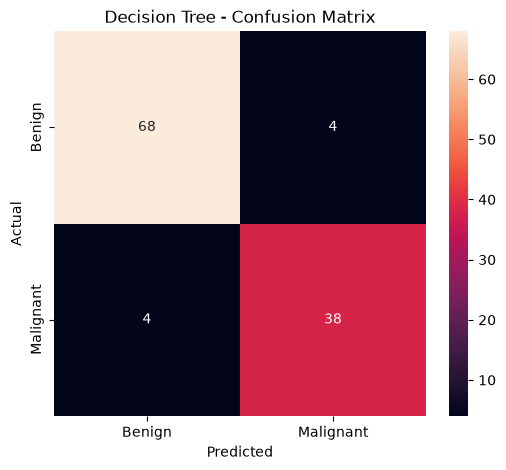
\includegraphics[width=0.55\linewidth]{figures/fig_cm_dt_baseline.png}
\caption{Confusion Matrix -- Decision Tree (untuned baseline, default hyperparameters)}
\end{figure}
\textbf{Inference:} The untuned baseline tree makes a mix of both false positives and false
negatives (roughly balanced), reflecting an unconstrained tree that has grown to depth 8 with 24
leaves -- deep enough to fit considerable training noise. Its overall test accuracy (0.9298) is
noticeably below the tuned tree's, indicating that the default configuration is not optimal for
this dataset.

\begin{figure}[H]
\centering
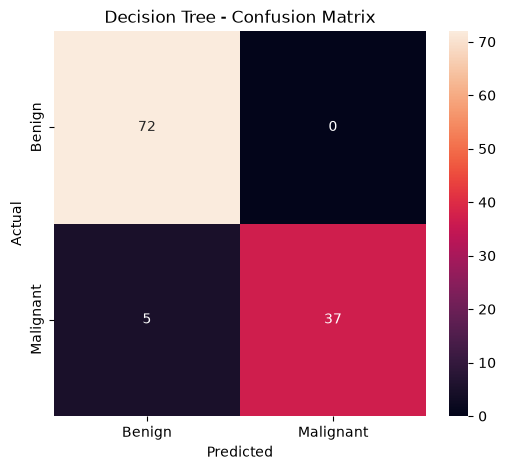
\includegraphics[width=0.48\linewidth]{figures/fig_cm_dt_tuned.png}
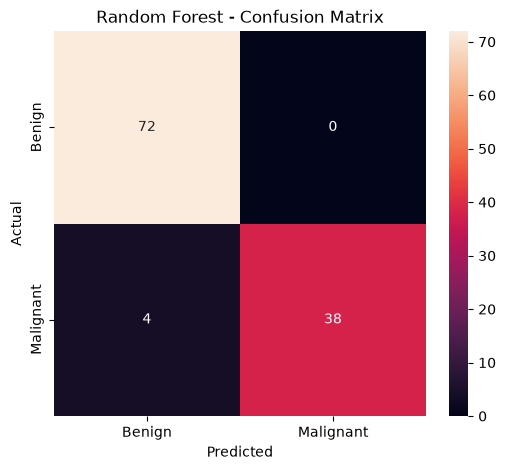
\includegraphics[width=0.48\linewidth]{figures/fig_cm_rf_tuned.png}
\caption{Confusion matrices -- tuned Decision Tree (left) and tuned Random Forest (right)}
\end{figure}
\textbf{Inference:} Both tuned models achieve perfect precision on the malignant class (zero false
positives -- no benign case is ever misclassified as malignant), but the Decision Tree misses more
true malignant cases (5 false negatives out of 42) than the Random Forest (4 false negatives).
Given that a false negative (missing a malignant tumor) is the more clinically costly error, the
Random Forest's slightly better recall (0.9048 vs. 0.8810) is a meaningful practical advantage
beyond what the accuracy difference alone suggests.

\begin{figure}[H]
\centering
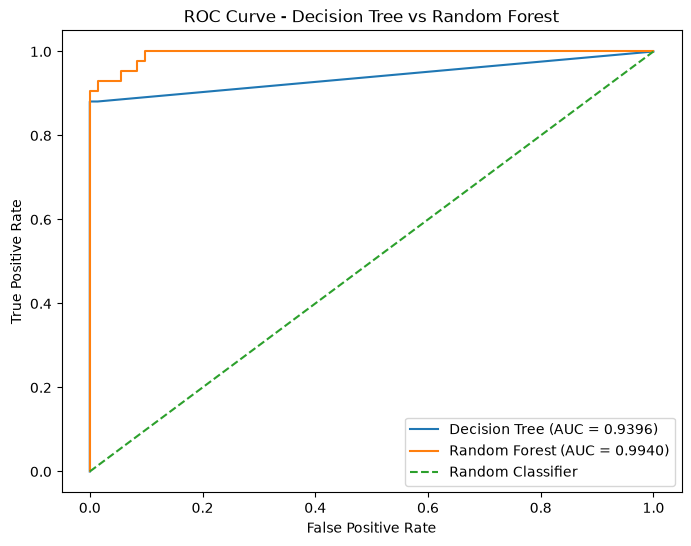
\includegraphics[width=0.7\linewidth]{figures/fig_roc_comparison.png}
\caption{ROC Curve -- Decision Tree vs. Random Forest}
\end{figure}
\textbf{Inference:} Random Forest's ROC curve dominates the Decision Tree's almost everywhere,
with a near-perfect AUC of 0.9940 compared to the tree's 0.9396. This gap is far larger than the
accuracy gap between the two models (0.9649 vs. 0.9561), showing that the Random Forest's
predicted probabilities are much better calibrated/ranked than the single tree's -- a benefit of
averaging many trees' probability estimates that a single tree's more discrete, step-function-like
probabilities cannot match.

\begin{figure}[H]
\centering
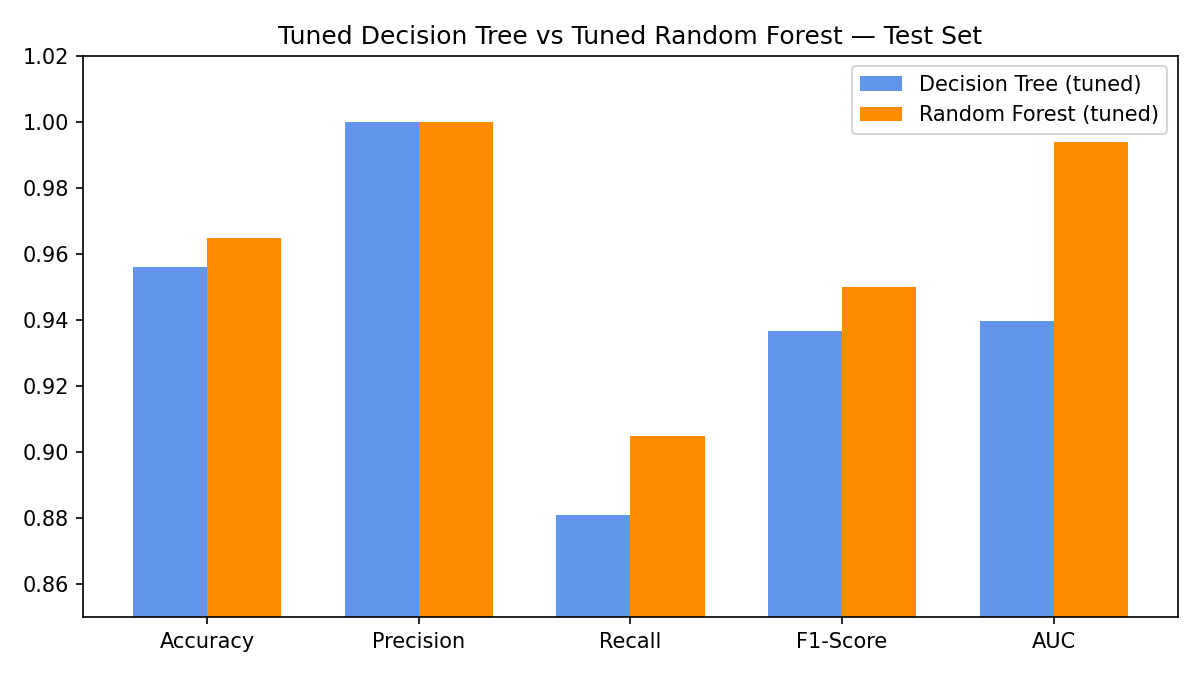
\includegraphics[width=0.85\linewidth]{figures/fig_final_comparison.png}
\caption{Tuned Decision Tree vs. tuned Random Forest -- all test-set metrics}
\end{figure}
\textbf{Inference:} Random Forest matches or exceeds Decision Tree on every metric, with the
largest gap in AUC and a smaller but consistent edge in accuracy, recall, and F1. Precision is
tied at a perfect 1.0 for both models, meaning the accuracy/F1/recall differences are driven
entirely by the malignant-class false negatives discussed above.

\begin{figure}[H]
\centering

\includegraphics[width=0.7\linewidth]{figures/fig_cv_folds.png}
\caption{5-fold cross-validation accuracy: Decision Tree vs. Random Forest}
\end{figure}
\textbf{Inference:} Random Forest outperforms the Decision Tree in every one of the 5 folds, with
a notably smaller spread (95.60--98.90\%) compared to the tree's wider spread (90.11--96.70\%).
This lower fold-to-fold variance is the direct, expected effect of bagging -- averaging over many
bootstrapped trees smooths out the instability that a single tree exhibits when the training data
changes slightly.

\begin{figure}[H]
\centering
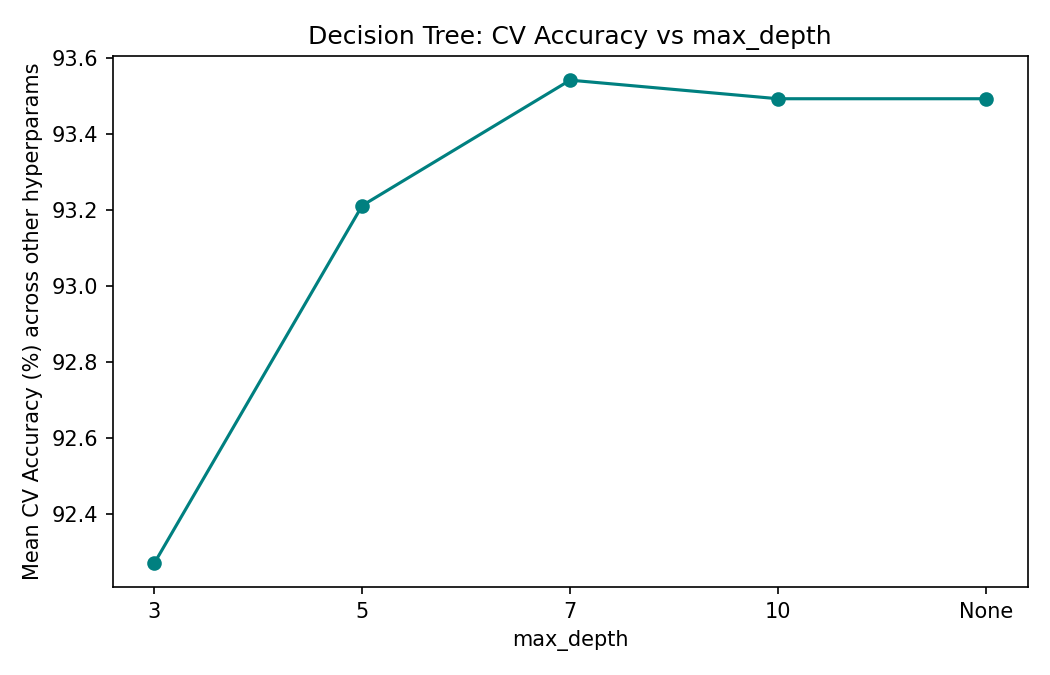
\includegraphics[width=0.7\linewidth]{figures/fig_dt_depth_accuracy.png}
\caption{Decision Tree: mean CV accuracy vs. max\_depth (averaged over all other
hyperparameter combinations)}
\end{figure}
\textbf{Inference:} Accuracy rises sharply from depth 3 to depth 7 (92.27\% to 93.54\%), then
plateaus and even dips slightly at depth 10 and beyond (including unbounded depth), showing that
this dataset needs only a moderate tree depth (around 7) to capture the signal, and unconstrained
depth offers no further benefit while adding overfitting risk -- consistent with the tied results
at depths 7/10/None seen in the Table~1 results above once \texttt{min\_samples\_split/leaf}
already limit further splitting.

\section{Discussion}

\subsection*{How does tree depth affect overfitting in Decision Trees?}
The depth-vs-accuracy analysis shows CV accuracy improving up to depth $\approx$7 and then
flattening, meaning depths beyond 7 add model capacity without improving (and slightly reducing)
generalization -- the classic overfitting signature. This is also visible in the baseline
(untuned, default) tree, which grew to depth 8 with 24 leaves and underperformed the tuned,
explicitly depth-limited tree on the test set.

\subsection*{Which hyperparameter had the greatest impact on performance?}
For the Decision Tree, \texttt{max\_depth} had the clearest effect (a 1.3 percentage-point swing
from depth 3 to the plateau at depth 7+), with \texttt{criterion=entropy} consistently
outperforming \texttt{gini} at matched depth in the top results. For Random Forest,
\texttt{bootstrap=False} combined with \texttt{max\_features=log2} dominated the top
configurations, suggesting that using the full (non-bootstrapped) training set per tree combined
with a smaller per-split feature subset generalized best on this particular dataset and split.

\subsection*{How does Random Forest improve generalization?}
By training many trees on bootstrapped samples (or, in this experiment's best configuration,
varied feature subsets) and averaging their votes, Random Forest reduces the variance component
of error without substantially increasing bias -- visible directly in this experiment's lower
fold-to-fold spread (95.60--98.90\% vs. 90.11--96.70\% for the single tree) and higher AUC
(0.9940 vs. 0.9396).

\subsection*{Did ensemble learning always improve performance? Why or why not?}
Yes, in every measured comparison here -- test accuracy, precision, recall, F1, AUC, and every
individual cross-validation fold -- Random Forest matched or exceeded the Decision Tree. This is
not guaranteed in general (ensembling can fail to help, or even hurt, if the base trees are too
correlated or the dataset is very small/simple), but for this 30-feature, 569-sample dataset with
substantial feature redundancy (88 highly correlated pairs), the random feature subsampling in
Random Forest had ample redundant signal to exploit for building diverse, decorrelated trees.

\section{Conclusion}
Both the tuned Decision Tree and tuned Random Forest achieve strong performance on the WDBC
breast-cancer classification task, but Random Forest is the clear winner: higher test accuracy
(0.9649 vs. 0.9561), higher recall on the clinically critical malignant class (0.9048 vs. 0.8810),
a substantially higher ROC-AUC (0.9940 vs. 0.9396), and lower variance across cross-validation
folds. Grid Search identified \texttt{max\_depth=7} (with \texttt{entropy}, \texttt{min\_samples\_
split=5}, \texttt{min\_samples\_leaf=2}) as optimal for the single tree, and \texttt{n\_estimators=
200}, \texttt{max\_depth=10}, \texttt{max\_features=log2}, \texttt{bootstrap=False} for the
forest -- both improving meaningfully over untuned defaults. The depth-vs-accuracy analysis
confirms the expected bias--variance story: shallow trees underfit, depth around 7 is near-optimal
for a single tree on this dataset, and further depth adds overfitting risk without benefit, a
risk that Random Forest's bagging/feature-subsampling largely neutralizes. For a real diagnostic
application, Random Forest's combination of higher recall and much better-calibrated probability
ranking (AUC) makes it the preferable model, at the cost of the interpretability advantage a
single Decision Tree retains.

\section{References}
\begin{enumerate}
\item Scikit-learn Developers, ``Decision Trees,'' scikit-learn documentation. [Online].
Available: \url{https://scikit-learn.org/stable/modules/tree.html}
\item Scikit-learn Developers, ``Ensemble methods -- Random Forests,'' scikit-learn
documentation. [Online]. Available:
\url{https://scikit-learn.org/stable/modules/ensemble.html#random-forests}
\item Scikit-learn Developers, ``Tuning the hyper-parameters of an estimator,'' scikit-learn
documentation. [Online]. Available:
\url{https://scikit-learn.org/stable/modules/grid_search.html}
\item UCI Machine Learning Repository, ``Breast Cancer Wisconsin (Diagnostic) Data Set.''
[Online]. Available: \url{https://archive.ics.uci.edu}
\end{enumerate}

\end{document}
